% \begin{itemize}
%     \item election prediction using candidate stats
%     \item election analysis using voter and candidate info
%     \item prediction using communication and how close 
%     \item Signed edge prediction and difficulties
% \end{itemize}
\section{Literature review}
\label{sec:literature-review}

The Wikipedia RfA process has been widely studied in various domains from many different perspectives such as those of the candidate, the voters, the community etc. In this section we discuss the existing work in this field.

Administrator is a highly coveted status on Wikipedia and there are many features than can be used to determine the worthiness of a candidate. Wikipedia themselves provide tools and guides\footnote{http://en.wikipedia.org/wiki/Wikipedia:GRFA} to help potential candidate assess their own electability. Wikipedia's \textit{admin score tool} as seen in Figure~\ref{fig:admin-score} uses features such as edit counts, pages created, age of account etc. Similarly, Burke et al. \cite{BurkeMoppingUp} utilized past RfAs to find features that correlate highly with success such as presence of edit summaries, politeness in user interactions and varied experience. Such tools and models are useful for finding potential nominees and understanding what the community values and respects. This however doesn't offer any insights into the dynamics that might play out in any particular election
\begin{figure}[h!]
    \centering
    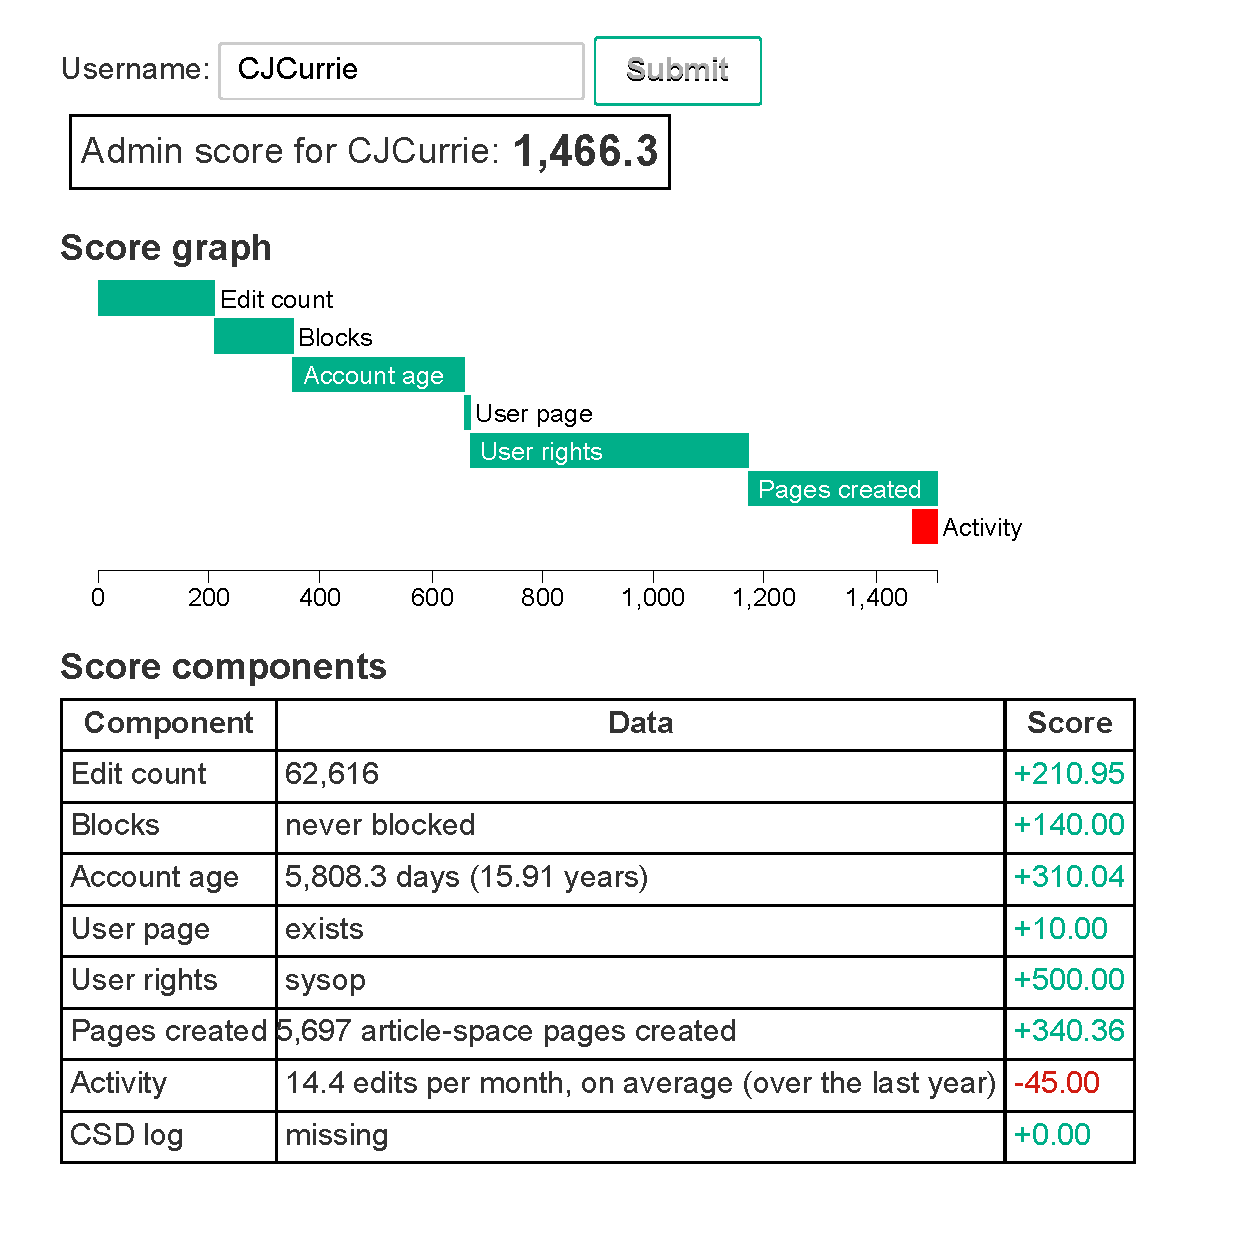
\includegraphics[width=\linewidth]{images/Asynchronous Admin Score.pdf}
    \caption{Admin score tool for user CJCurrie and it's breakdown}
    \label{fig:admin-score}
\end{figure}

Leskovec et al. provide a thorough analysis of the election from the perspective of the voter. They show that the voters make decisions based on \textit{relative assessment} of merit and degree of correspondence with the candidate. Elections do not follow a \textit{herd mentality} and standard information cascades. We see an interesting result that voters have diverse personal response functions as well as admin and non-admin patterns of voting differ. \cite{leskovec2010governance} We get a detailed picture of the temporal dynamics in a RfA.

As the votes in an RfA election can be positive or negative they can form a \textit{signed network} which has been studied and analyzed in great detail. We see that the Wikipedia RfA network has more compliance with status theory compared to balance theory in Leskovec et al. \cite{leskovecSigned}. When Leskovec et al. try and use these signed structural properties to predict edges in \cite{leskovecPredicting}, they see that the predictive accuracy is poor for Wikipedia RfA network compared to the other networks used. However as signed edge prediction methods are designed to work with any generic signed network, they tend to discard information that RfAs are elections and play out in a timely manner. Also predicting a single edge i.e a vote does not increase the accuracy in predicting the result of an election.   

The work of Desai et al. \cite{desai2014result} is related closely with the contributions presented in this paper. They use linear models for regression and classification to identify a core of \textit{influential voters} through feature selection. Using a set of 40 most influential voters they are able to predict the result of an election with a high accuracy. They also collect additional network features of the voters independent from the elections. Their results do not improve significantly in using the additional features in predicting election results. These results show that there are a group of influential voters that determine elections. This will be more evident when we analyze the dataset in coming sections.
